\documentclass{article}
\usepackage[final]{common/neurips_2022}
\usepackage[nottoc,numbib]{tocbibind}
\usepackage[utf8]{inputenc} % allow utf-8 input
\usepackage[T1]{fontenc}    % use 8-bit T1 fonts
\usepackage{hyperref}       % hyperlinks
\usepackage{url}            % simple URL typesetting
\usepackage{booktabs}       % professional-quality tables
\usepackage{amsfonts}       % blackboard math symbols
\usepackage{nicefrac}       % compact symbols for 1/2, etc.
\usepackage{microtype}      % microtypography
\usepackage{xcolor}         % colors

\usepackage{graphicx}
\usepackage{amsmath}
\usepackage{float}

\title{Personalized Recipe Recommendation Using Heterogeneous Graphs}

\author{%
  Nicholas DeGroot \\
  Halıcıoğlu Data Science Institute \\
  University of California, San Diego \\
  La Jolla, CA 92122 \\
  \texttt{ndegroot@ucsd.edu}
}


\begin{document}


\maketitle


\begin{abstract}
  Recent social and economic trends have led to a rise in the number of people cooking at home. However, many people struggle to find recipes that fit their current culinary goals. We present a novel approach to help users find personalized recipes using heterogeneous graphs. We use a graph data structure to represent recipes and reviews, and leverage the graph structure to capture the relationships between recipes and users. We then use a graph neural network to learn a representation of the graph that can be used to recommend recipes to users. We evaluate our approach on a dataset of \verb|food.com| reviews and show that our model outperforms a baseline model that does not leverage the graph structure.
\end{abstract}


\section{Introduction}
% There are three pieces to an introduction section:
% 
% 1. An introductory paragraph. The first paragraph in your introduction will start by introducing the context in which your project is relevant. It will then state the problem that you’re trying to solve, and summarize some of your key results and their implications.
% 
% 2/ A literature review and discussion of prior work. Here, you’ll provide context on what has been attempted in the past in the realm of your problem. This will both set up the context in which your problem exists and shed light on why your approach is different.
% 
% 3. A data description (this is a data science capstone, after all).
% 
% If you’re in a data-focused domain, you should describe why the data you’re using will help address the problem at hand.
% If you’re in a methods-focused domain (that is, a domain in which you’re developing new methods), you should describe the kinds of data that your methods are applicable to. For instance, if you’re developing methods for using convolutional neural networks with graphs, you should describe why graph-based data is useful in the real-world.


We've all been there. It's been a long day of work, but you're finally home and ready to cook. The only problem: you have no idea what to make.

\begin{itemize}
  \item You could fall back on some classics, but it feels like you've been eating the same thing for weeks.
  \item You could go out to eat, but that's expensive and you're trying to save money.
  \item You could order takeout, but that's unhealthy and you're trying to eat better.
\end{itemize}

What's needed is a way to find new recipes that you'll actually enjoy, personalized to the things you already have on hand. Users should be able to open up an app, see what's been scheduled for the day, and start cooking. Should users not like what's scheduled, it should be easy to swap out recipes for something else and incorporate that feedback into future meals.

To my knowledge, nothing like this is available on the market. Existing services generally fall within one of two categories.

\begin{itemize}

  \item \textbf{Recipe Aggregators:} These services provide a collection of recipes that users can browse and search. Users are expected to find the recipes they want to cook themselves. Some services such as Yummly have integrated personalized search recommendations to make finding recipes easier, yet require users to manually build out their meal plans.
        
  \item \textbf{Meal Kits:} These services provide pre-portioned ingredients and recipes for users to cook. Users select from pre-determined plans (such as Meat \& Veggies) and are sent a box of pre-portioned ingredients with their associated recipe each week. Minor customization is possible, but users are locked into a limited number of recipes. These services can become quite expensive and often require users to commit to a subscription.
        
\end{itemize}

Each service has its own strengths and weaknesses. Recipe aggregators are free and allow users to cook whatever they want, but require users to do all the work of finding recipes and building out meal plans. Meal kits are convenient and allow users to cook without having to think about it, but are expensive and require users to commit to a subscription.

This project is the first step to creating the system that combines the best of both worlds. We propose a solution to the core piece powering it all: the recommendation system.

\section{Methods}
% This section often goes by different names, e.g. experimental design, and sometimes appears at the start of the “Results” section of a paper rather than as its own section (as we saw in the chart above). Regardless of its title, the purpose of this section is to describe the steps that you took to produce the results you’ll discuss in the following section. It should contain enough details for a reader to be able to understand what you did, without containing so much detail that it distracts from the storyline – leave ultra-fine details for the appendix.

% If your project involves developing multiple models that are very different, you may want to dedicate a separate section to each one. This may apply, for instance, if you used two different approaches to solve your overarching problem, or if you used different models to label data and to train a classifier.

To build out our recipe recommendation system, we used an existing dataset published by \citet{recipegen} of \verb|food.com| reviews. After cleaning the dataset and parsing it into a graph data structure, we were left with the following nodes/edges:

% https://mermaid.live/edit#pako:eNqNkl9rwjAUxb9KyNMGFabSOosKjjkQOgXt9lQoWXOtgTYp-eMQ6XdfajvU2sHuS8vv3NzkHs4JJ4IC9nGSEaVeGUklySOObFEmIdFMcLQJIl6zcxf6UCBPNahqMlnZGbPZhTw8ohWaosHAc9zRU83L6wkbSFgB6F9Dhn3HG45-X1DVchWinHGjQd1CHisNxRV8C9bzECUkE5LBHddCkyzeER0X9NAWlUmJ7BQEZSbvUgopNDDeeYhoI4kG-td1CZFfYn-kVZO6NJS3zm_gwOD71rcFTe98i8PNfFm5NxoPHM_1WurnPJj2vbHz7Lrtc4tt2Ehe23L7NMbTC3tZrwPEVKwlYfweH0jW0QtKtzar0oR6vWa3mjV7nmmVFOzgHGROGLVRPW8fYb2HHCLs218KO2IyHeGIl7aVGC22R55gX0sDDjYFta424cb-jmTKUqBMC_nexL_6lD85pN3_
\begin{figure}[h]
  \centering
  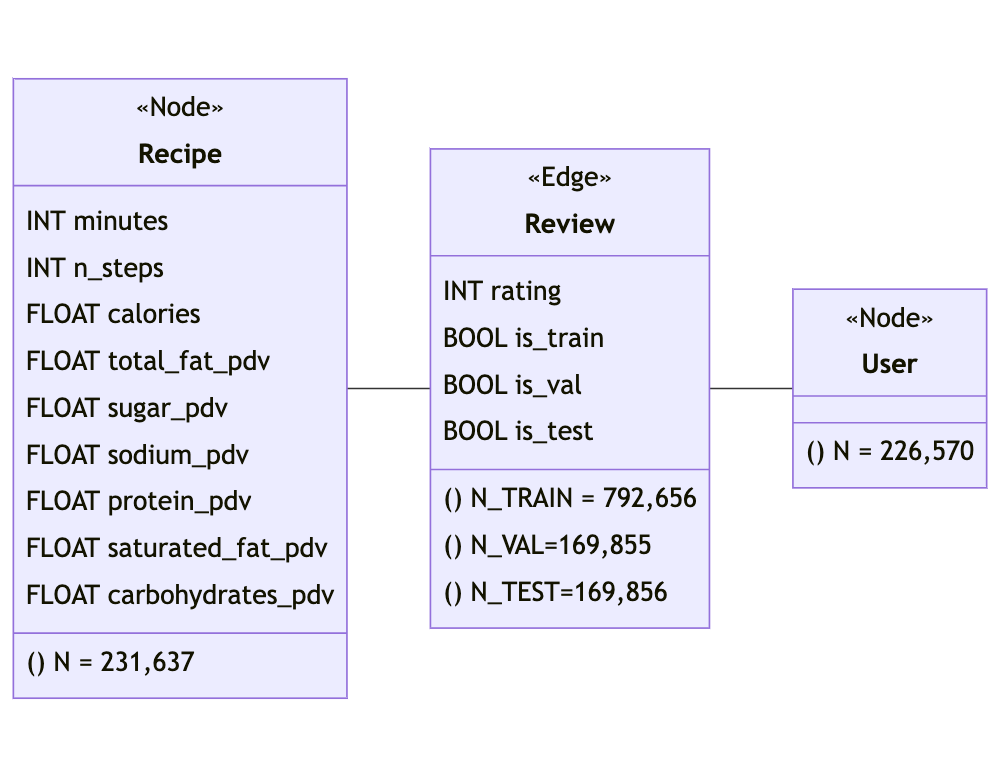
\includegraphics[height=150px]{figures/schema.png}
  \caption{Graph structure of the recipe dataset}
  \label{fig:recipe_graph}
\end{figure}

This data was then uploaded to TigerGraph, a graph database that allows for fast and scalable storage of graph databases. Their schema system was particularly useful for this project, as it allowed us to easily define the heterogeneous structure of the graph directly inside the database.

We then downloaded the data into a Python environment and trained a variety of graph-based models.

\subsection{K-Means Collaborative Filtering}

Our first attempt at recommending recipes to users was to use a K-Means collaborative filtering model. K-Means collaborative filtering is a classical algorithm that recommends items to users under the assumption that users with similar tastes will like similar items.

The model works by first computing a similarity score between users. We chose to use the pearson correlation coefficient as our similarity metric, due to its ability to handle non-centered ratings (such as the 1-5 ratings we used). The model then predicts a score for each user-recipe interaction based on a weighted average of the ratings of users.

$$
  \text{Recipe Score}(u, r)
  = \mu_{u} + \frac{
    \sum_{u'} \text{Similarity}(u, u')
    \cdot (\text{Rating}(u', r) - \mu_{u'})
  }{
    \sum_{u'} \text{Similarity}(u, u')
  }
$$

Recommendations are then as simple as sorting the recipes by their predicted score and choosing the top $k$.

We implemented the algorithm in two ways for this project.
\begin{enumerate}
  \item \verb|surprise|: An open-source Python library that implements a variety of recommendation algorithms \citep{suprise}. Their implementation of Centered K-NN closely mirrors the algorithm described above, thus making it an easy choice for our first model.
  \item \verb|GSQL|: We also implemented the model inside TigerGraph using GSQL. This allowed us to run recommendations \textit{directly inside the database}, allowing for lightning fast recommendations suitable for real-time applications.
\end{enumerate}

One important distinction between our implementations and many others is that we did not filter out recipes that users have already interacted with. We decided to do this because we wanted to be able to recommend recipes that users have already interacted with, but may have not tried in awhile. This is particularly important to note when considering the results of our prior user research, which suggested that users generally prefer to cook recipes they've already cooked before.

\subsection{Graph Neural Networks}

While a pure collaborative filtering model is able to capture some of the relationships between users and recipes, it's unable to capture more complex relationships. For example, if a user has a history of liking Indian food, we would like our system to recommend other Indian recipes (regardless of what "similar users" are having). To accomplish this, we next experimented with graph neural networks (GNNs).

Two libraries were used to implement the GNNs created in this project:
\begin{itemize}
  \item \verb|PyTorch|: A popular deep learning framework \citep{pytorch}. This library was chosen because it is well documented and has a large community of users.
  \item \verb|PyTorch Geometric|: A library that extends \verb|PyTorch| to support graph neural networks \citep{pyg}. This library was chosen for its natural integration with PyTorch.
\end{itemize}

\subsubsection{LightGCN}

After researching a variety of GNN architectures, we decided to expand on the LightGCN model architecture. LightGCN is a GNN architecture created by \citet{lightgcn} specifically designed for recommendation tasks.

At its core, LightGCN is similar to traditional matrix factorization methods. It uses a user embedding matrix $U$ and a recipe embedding matrix $R$ to represent the latent features of users and recipes. The score for a particular user-recipe interaction is then computed as the dot product of the user and recipe embeddings.

$$
  \text{Recipe Score}(u, r) = U_u^TR_r
$$

This equation can be thought of as the sum of a user's preferences for each feature multiplied by the recipe's affinity for that feature. For example, if a latent feature corresponded with "spice", users who like spicy food would have a high value for that feature as would recipes that are spicy. Thus, the resulting score for such a user-recipe interaction would be high.

The difference between LightGCN and traditional matrix factorization methods is that LightGCN learns the embedding matrices in context of the graph. Before computing the score for a user-recipe interaction, LightGCN first passes the user and recipe embeddings through a "light graph convolution" layer. This layer uses the features of each node's neighbor(s) in a normalized weighted sum to compute the new embedding for that node.

$$
  \begin{aligned}
    U_u & \gets \sum_{r \in N(u)} \frac{1}{\sqrt{d_u d_r}} R_r \\
    R_r & \gets \sum_{u \in N(r)} \frac{1}{\sqrt{d_r d_u}} U_u
  \end{aligned}
$$

This process can then be repeated and averaged to allow for more complex modeling.

During training, we utilized Baysean Personalized Ranking (BPR) loss to optimize the each of the embedding matrices. BPR loss is a loss function that is commonly used for recommendation tasks. It is designed to maximize the score of positive/real user-recipe interactions and minimize the score of negative/fake user-recipe interactions. To help prevent overfitting, we also added a regularization term to the loss function.

$$
  \begin{aligned}
    \text{BPR Loss}       & = -\frac{1}{N} \sum_{(u, r, r') \in D} \log \sigma(U_u^TR_r - U_u^TR_{r'})             \\
    \text{Regularization} & = \lambda \cdot \left( \sum_{u} \Vert U_u \Vert^2 + \sum_{r} \Vert R_r \Vert^2 \right)
  \end{aligned}
$$

\subsubsection{RecGCN}

While LightGCN is able to capture a lot of underlying relationships, it neglects a variety of information we have available to us.

\begin{itemize}
  \item \textbf{Recipe Features}: LightGCN only uses the user and recipe embeddings to compute the score for a user-recipe interaction. However, we have a variety of features available to us for each recipe, such as nutritional information and cooking time.
  \item \textbf{Review Rating}: LightGCN only normalizes the weights of each interaction by the degree of each node. However, we have access to the actual rating that each user gave to each recipe, which indicates how strong the interaction actually was.
\end{itemize}

To address these issues, we propose a new GNN architecture called RecGCN. RecGCN is a slight modification of LightGCN with two main changes. First, we scale the graph convolution layer by the review's score.

$$
  \begin{aligned}
    U_u & \gets \sum_{r \in N(u)} \frac{\text{Review}(u, r)}{\sqrt{d_u d_r}} R_r \\
    R_r & \gets \sum_{u \in N(r)} \frac{\text{Review}(u, r)}{\sqrt{d_r d_u}} U_u
  \end{aligned}
$$

Second, we define a recipe feature matrix $F$. This matrix contains a row for each recipe, and a column for each feature. We have two options for how to use this matrix.

\begin{itemize}
  \item \textbf{Opposite Embedding}: We can substitute the recipe embedding matrix $R$ with the recipe feature matrix $F$. Due to the nature of the graph convolution layer, we also need to redefine the user embedding matrix $U$ to have the same number of columns as $F$. This will force the model to learn embeddings for the user for each recipe-defined feature.
  \item \textbf{Combination}: We can concatenate the recipe embedding matrix $R$ with the recipe feature matrix $F$. This will allow the model to learn embeddings for each recipe-defined feature, as well as latent embeddings for the recipe as a whole. Due to the nature of the graph convolution layer, we also need to redefine the user embedding matrix $U$ to have the same number of columns as $F$ + $R$.
\end{itemize}


\section{Results}

In this section, we compare the results of our various models. All experiments were performed on a desktop workstation with a AMD Ryzen 9 5900X CPU and Nvidia RTX 3080 GPU.

All models were trained solely on interactions with \verb|is_train = True|. For models that support iterative training, we saved the best model based on its Precision@10 performance on interactions with \verb|is_validation = True|. Models were finally evaluated on interactions with \verb|is_test = True|. The results are shown in Figure \ref{fig:model_eval} for recommendations at several $k$ values.

\begin{figure}[h]
  \centering
  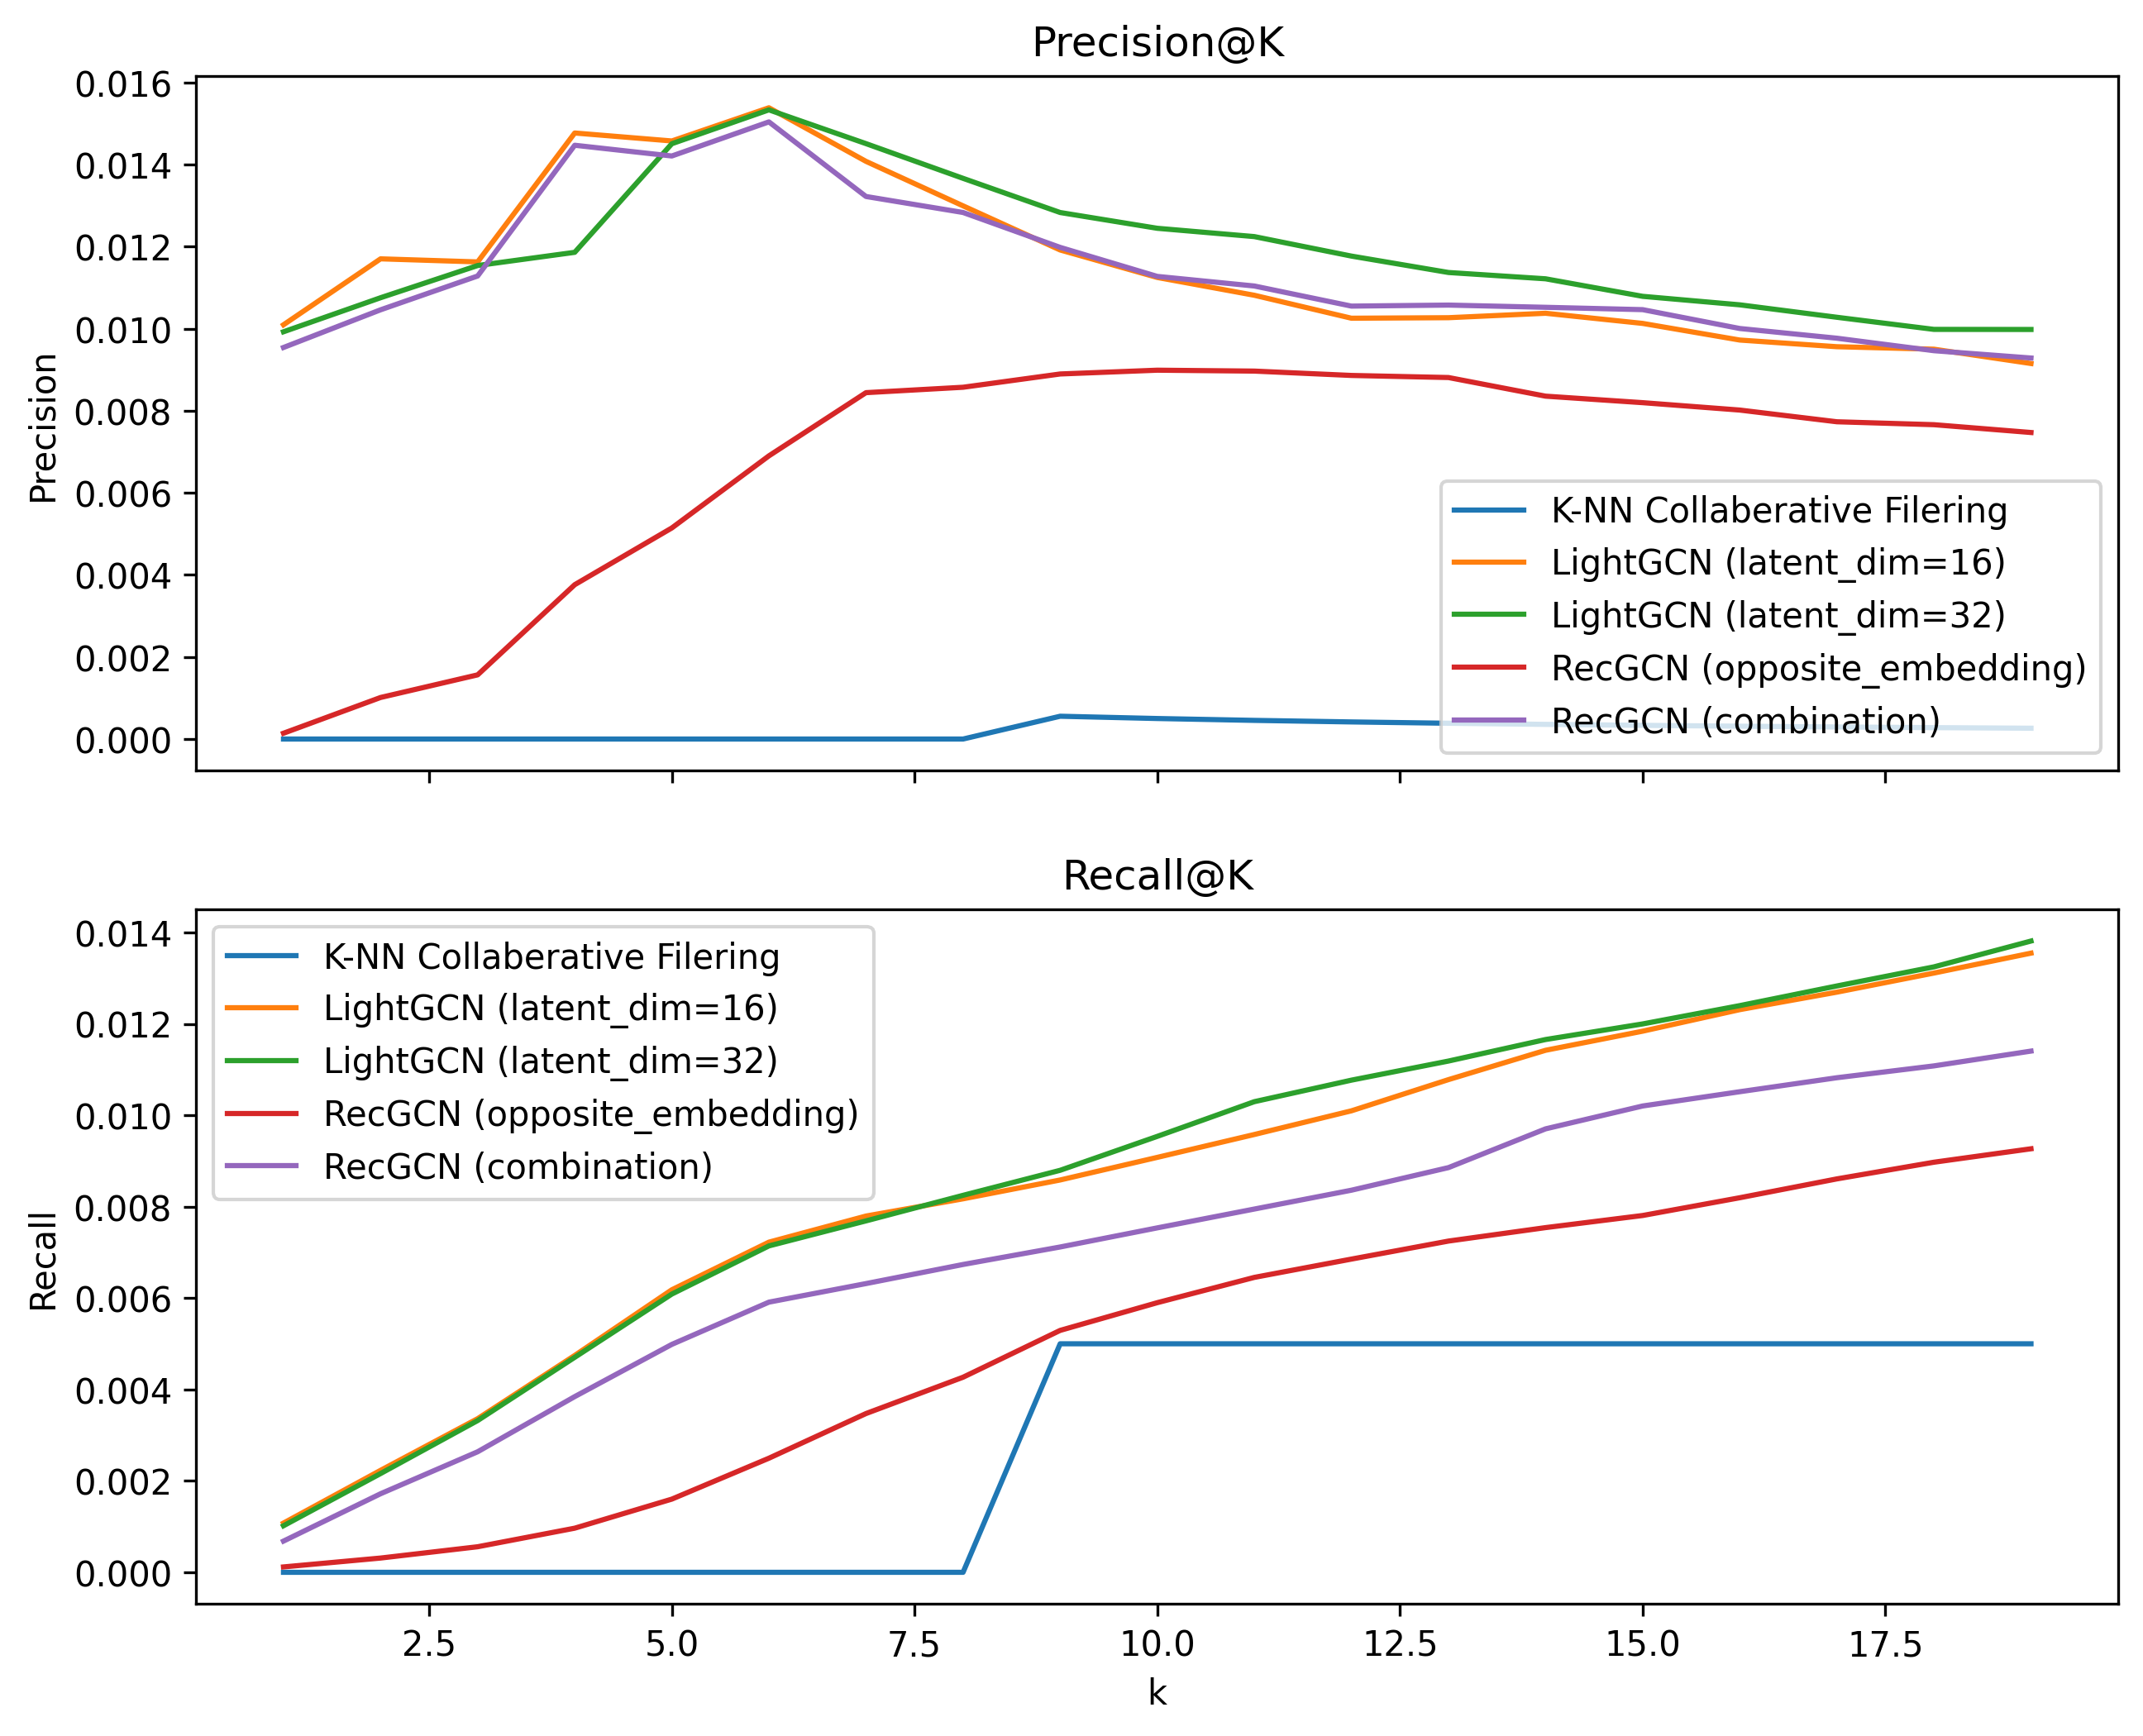
\includegraphics[width=0.75\linewidth]{figures/model_eval.png}
  \caption{Model results on the test set}
  \label{fig:model_eval}
\end{figure}

The first thing to note is that K-NN collaborative filtering did not work well with this dataset, performing far worse then every GNN model. Further research reveals that this may be due to the fact that the dataset is extremely sparse, with only $\approx 52\%$ of test users and $\approx 79\%$ of test recipes even showing up in the training set. With both needed to even produce a recommendation, this results in a very small number of possible interactions.

This finding also explains LightGCN's great performance, which is comparable to the original LightGCN paper's results on the Amazon-Book dataset (another sparse dataset).

Surprisingly, LightGCN performed well enough to outperform every version of RecGCN. We believe this may be similar to the reason LightGCN outperformed many of its predecessors: the simplicity of the architecture. One common issue we ran into during training is that our models quickly began to overfit the data, resulting in poor performance on the validation set. Simpler models are able to sidestep this issue through their inability to model complex relationships.

\begin{figure}[h]
  \centering
  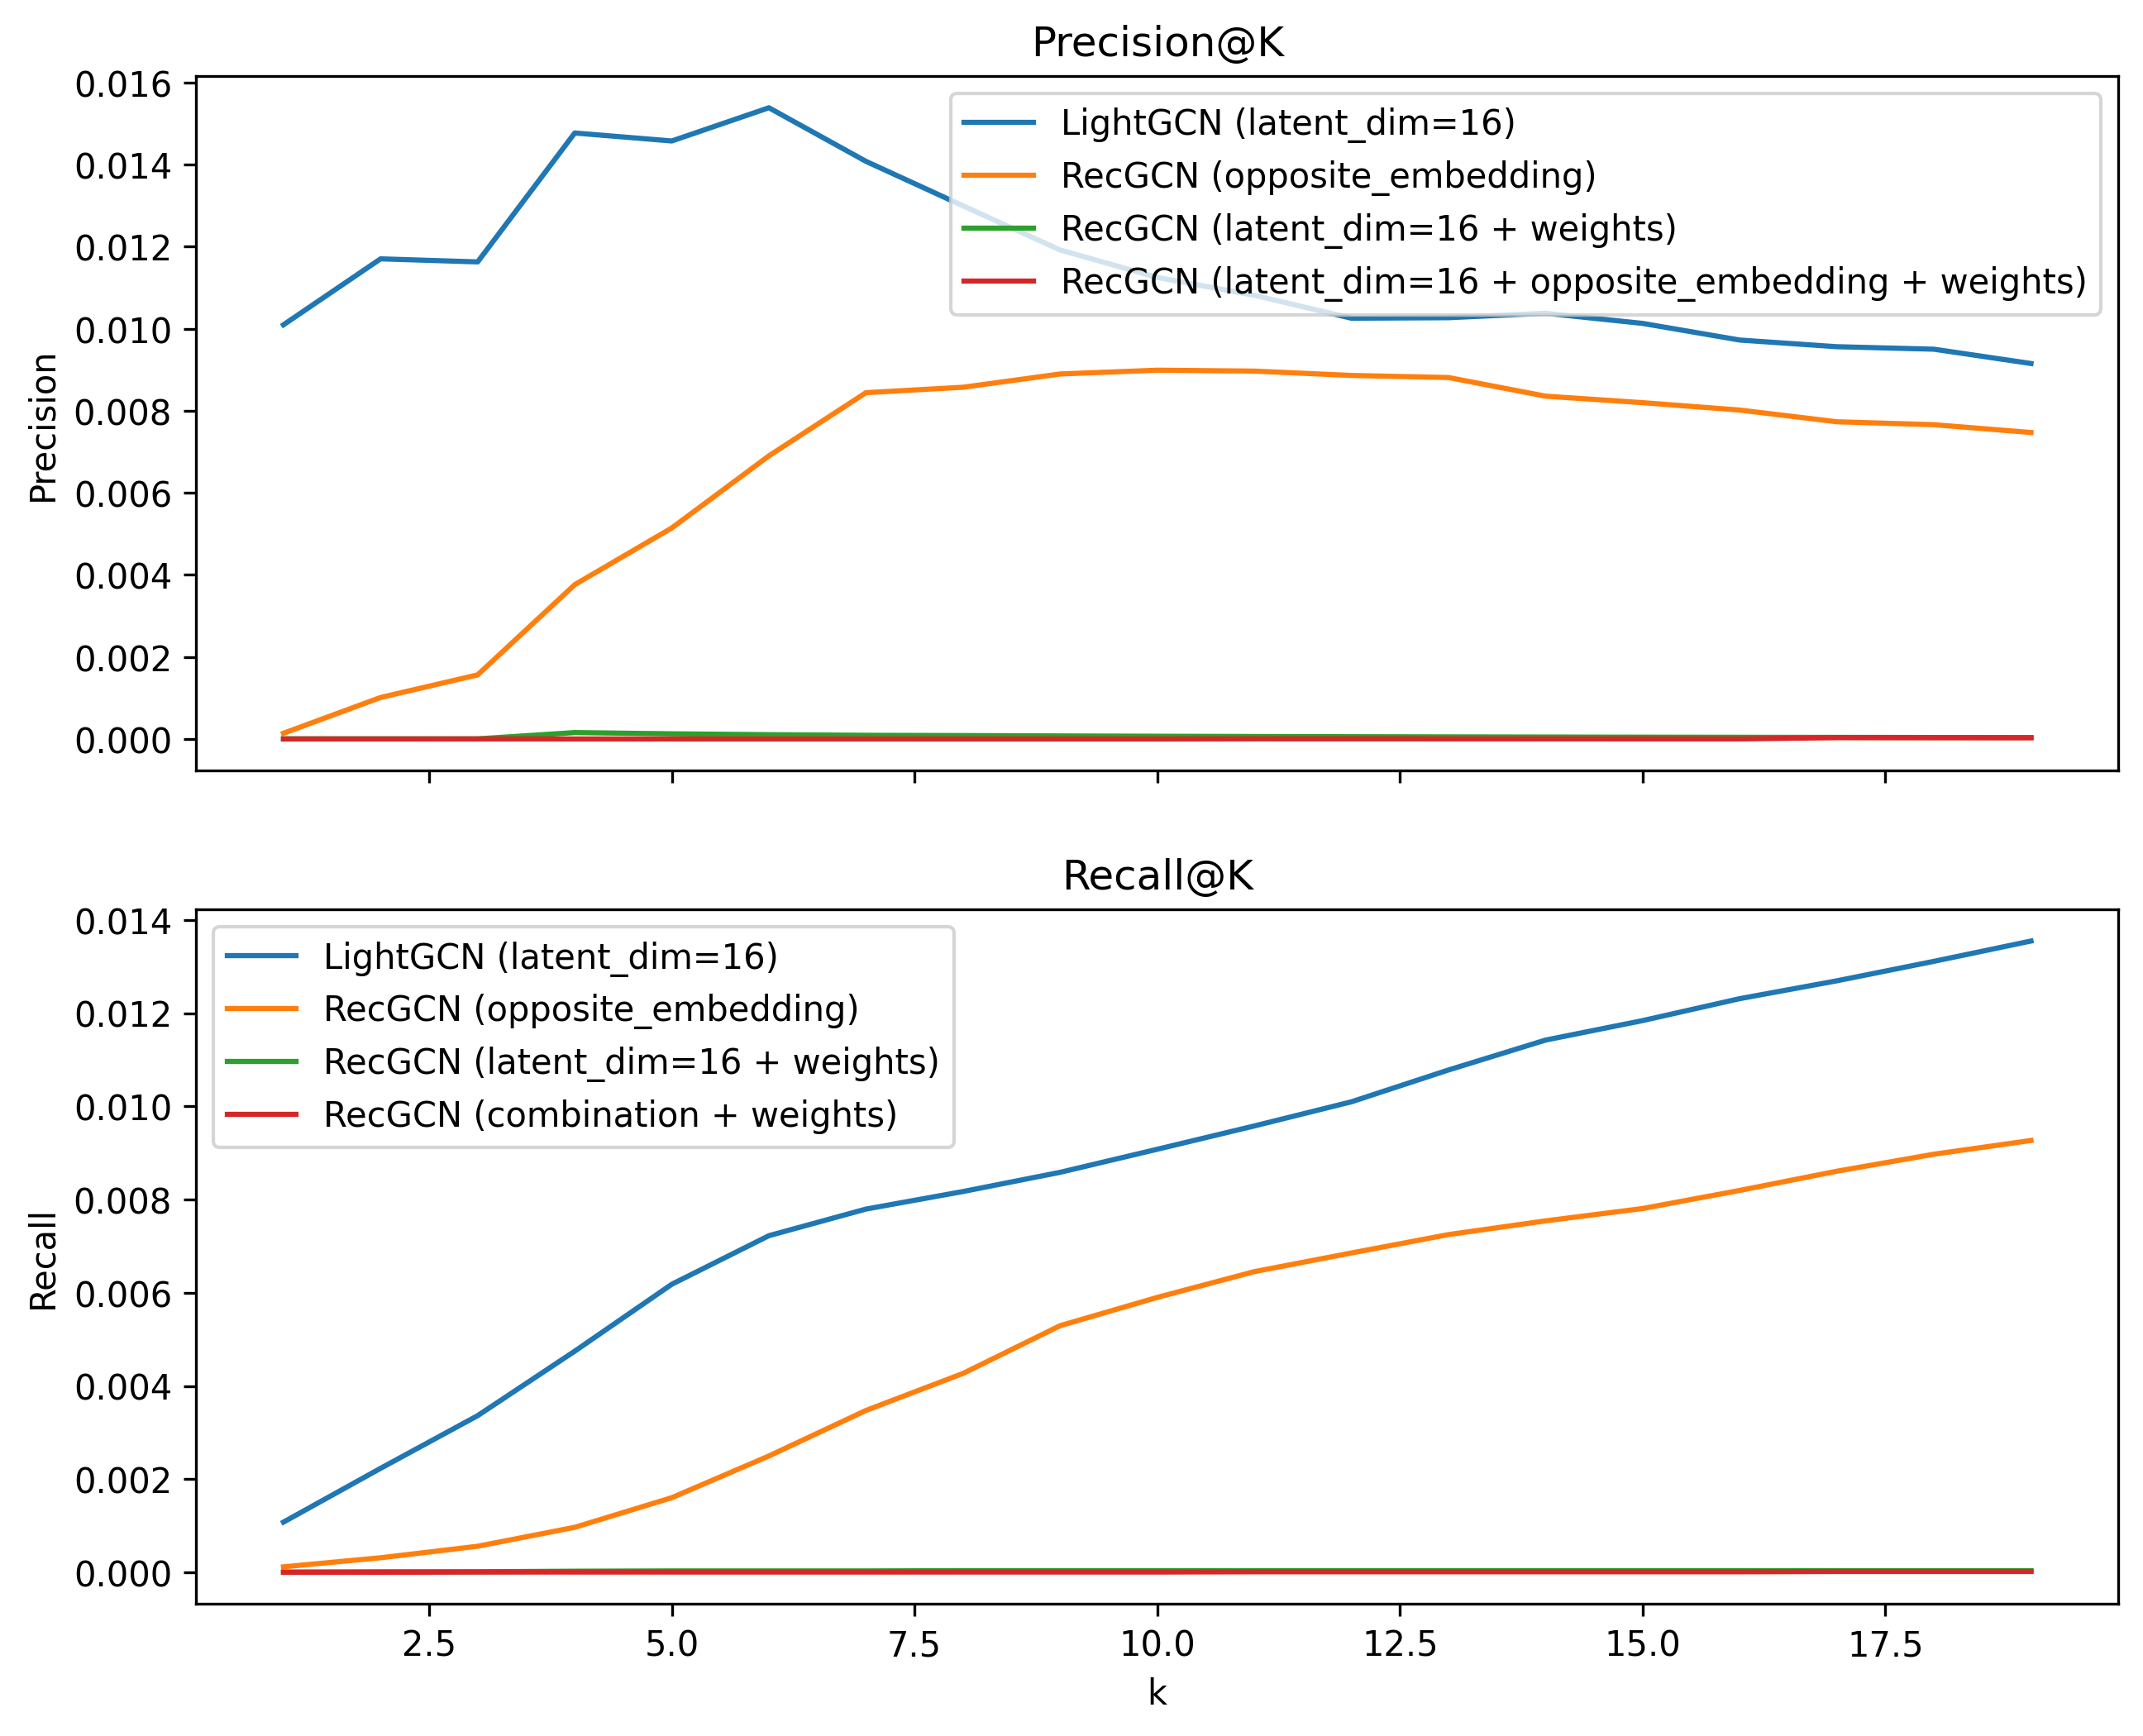
\includegraphics[width=0.75\linewidth]{figures/flag_eval.png}
  \caption{RecGCN changes on the test set}
  \label{fig:flag_eval}
\end{figure}

In order to further investigate how each RecGCN alteration affected the model, we also performed an analysis on each of the changes we made. The results are shown in Figure \ref{fig:flag_eval}.

The first thing to note is that the addition of review weights destroyed the model's performance. We believe this may be due to multiple high reviews exponentially scaling certain embeddings, resulting in a complex relationship that the model is unable to model. We talk more about possible solutions to this issue in the future work section.

The second thing to note is that the addition of recipe features did not have a significant impact on the model's performance. If anything, it slightly \textit{decreased} the model's performance. We believe this may be due to the fact that the features we have available to us aren't as descriptive as the latent variables learned by the model. For example, LightGCN may learn that a user prefer's "healthier" recipes, but a opposite embedding RecGCN model can only learn whether a user likes recipes low in fat. 

\section{Conclusion \& Future Work}

At the end of the day, the success of this project is based on whether or not it can be used to solve the problem of meal planning. To that end, we believe that our models are able to provide a good starting point for a full meal planning system. The recommendation engines we built are able to recommend recipes that a user is likely to enjoy, particularly if the rest of the system is built with the weaknesses we found in mind. We envision a system that allows users to reject recipes for their weekly meal plan, and then have the system automatically recommend new recipes to replace them. Our best model is able to recommend a recipe the user enjoys within roughly 50 iterations \textit{even with a relatively small history}.

The best part of such a system is that those rejections can be used to improve the recommendation engine. The system can learn from the user's rejections and use that information to improve the recommendations in the future. This not only results in better recipes for the user, but solves the sparsity problem that we ran into with all of our models!

\begin{figure}[h]
  \centering
  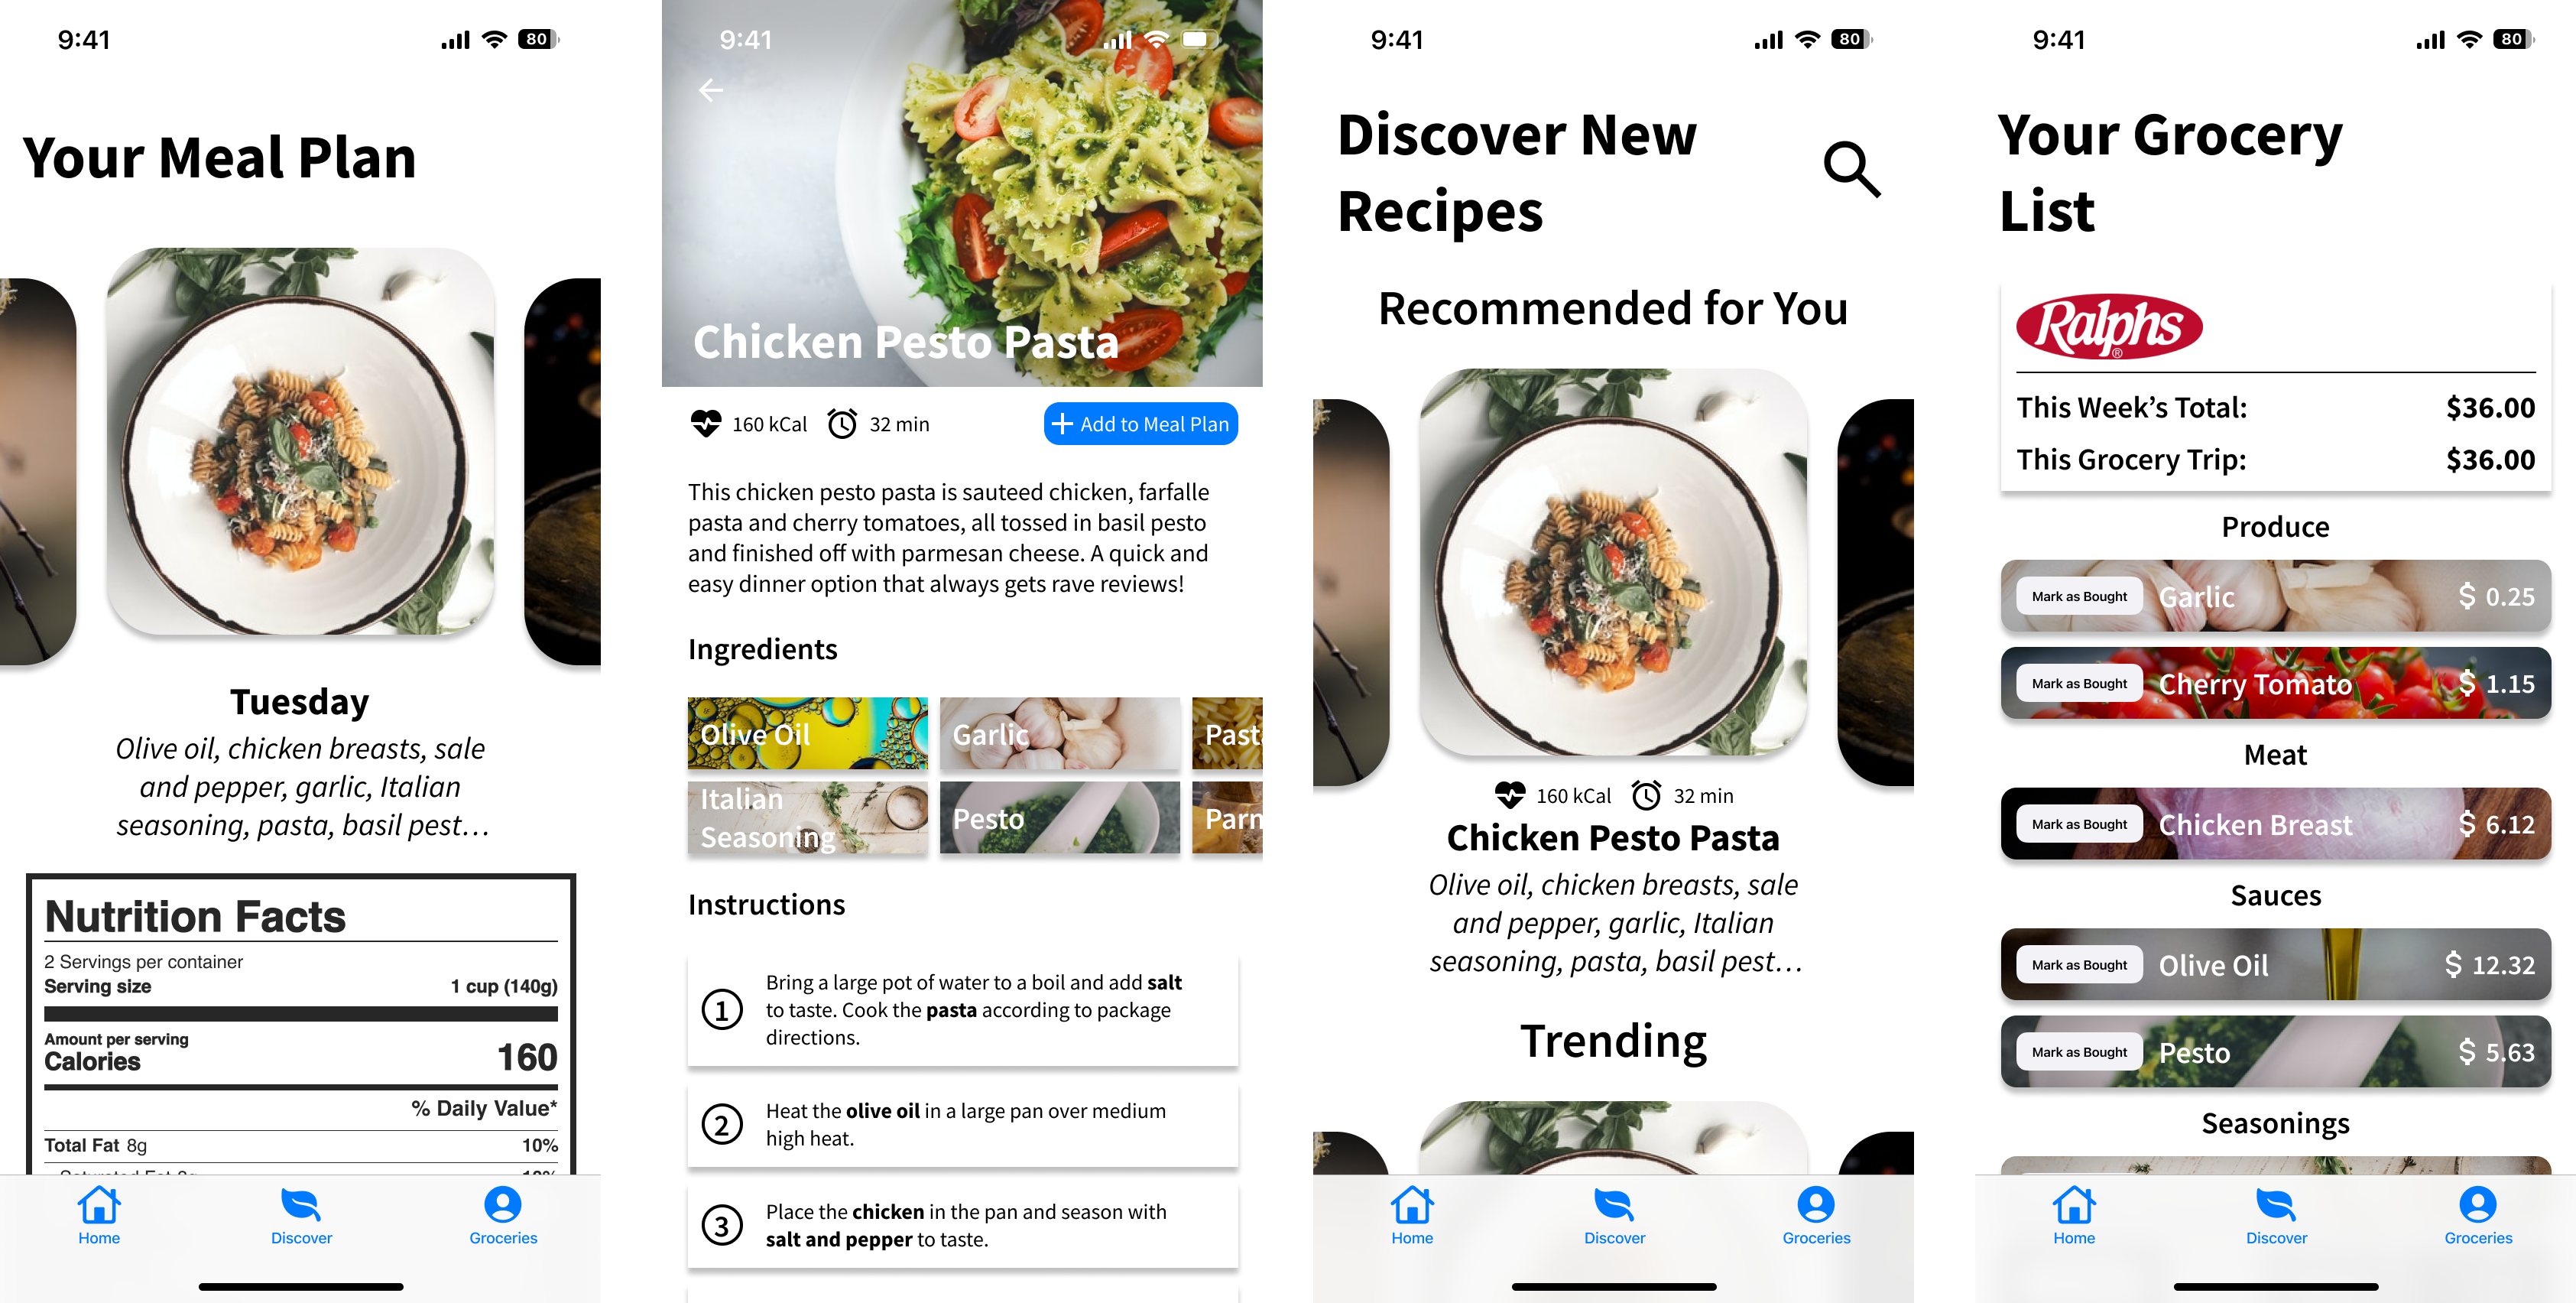
\includegraphics[height=200px]{figures/ux.png}
  \caption{Current UX Mockup}
  \label{fig:ux}
\end{figure}

We plan to continue this work in a commercial setting. We believe that this project can be a core component of a full system that helps people save time and money by automating the process of meal planning and grocery shopping.

Future work includes:
\begin{itemize}
  \item \textbf{User Interface}: Performing a user study to determine the best way to present the recommendations to the user. One early prototype of the user interface is shown in Figure \ref{fig:ux}.
  \item \textbf{Software Development}: Developing the core app to be used by the user.
  \item \textbf{Alternative Recommendation Methods}: Investigate other recommendation methods, such as Facebook's Deep Learning Recommendation Model (DLRM) \citep{dlrm}.
\end{itemize}

As for the research side of this project, we plan to continue investigating the following:

\begin{itemize}
  \item \textbf{RecGCN Review Weighting}: Investigate alternative methods of weighting the reviews, such scaling the weights by the user's average or normalizing the new edge weight by the sum of the reviews.
  \item \textbf{Recipe Features}: Investigate alternative methods of using recipe features, such as using a neural network to learn the best way to combine the features with the embeddings.
\end{itemize}

%%%%%%%%%%%%%%%%%%%%%%%%%%%%%%%%%%%%%%%%%%%%%%%%%%%%%%%%%%%%


\bibliographystyle{dinat}
\bibliography{citations}

% \appendix
% \section{Appendix}

\end{document}